Our app consists of a web app made with the React for Javascript, a backend app made with the Spring framework for Java, a MongoDB database, as well as an API for the simulator written in Go.
The Spring-backend exposes a REST interface for interacting with the database. The interface allows for user registration, logging in, getting and posting tweets, and so on.

The web app uses this REST interface to provide its functionality and display a graphical interface in a browser. The flow of interactions between a user and MiniTwit is illustrated in Figure \ref{fig:informal_flow}

\begin{figure}[h]
    \centering
    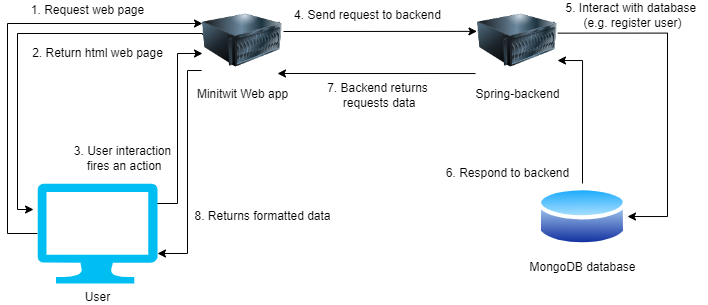
\includegraphics[width=\textwidth]{images/Minitwit flow.drawio.png}
    \caption{Flow of requests from a user}
    \label{fig:informal_flow}
\end{figure}

The Simulator API functions as an intermediate layer, translating and forwarding requests from the simulator to the Spring-backend. The flow of interactions is illustrated in Figure \ref{fig:informal_simulator}

\begin{figure}[h]
    \centering
    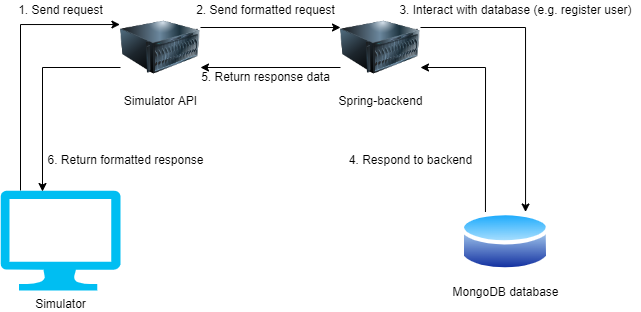
\includegraphics[width=\textwidth]{images/Minitwit simulator.drawio.png}
    \caption{Flow of requests from the simulator}
    \label{fig:informal_simulator}
\end{figure}
